\section{Day 8: Continuous Functions and Infinite Products (Sep. 26, 2024)}
Outfit of the day! Sniper monkey 0-2-5 outfit!!!! very demure, very mindful
\begin{figure}[h]
    \centering
    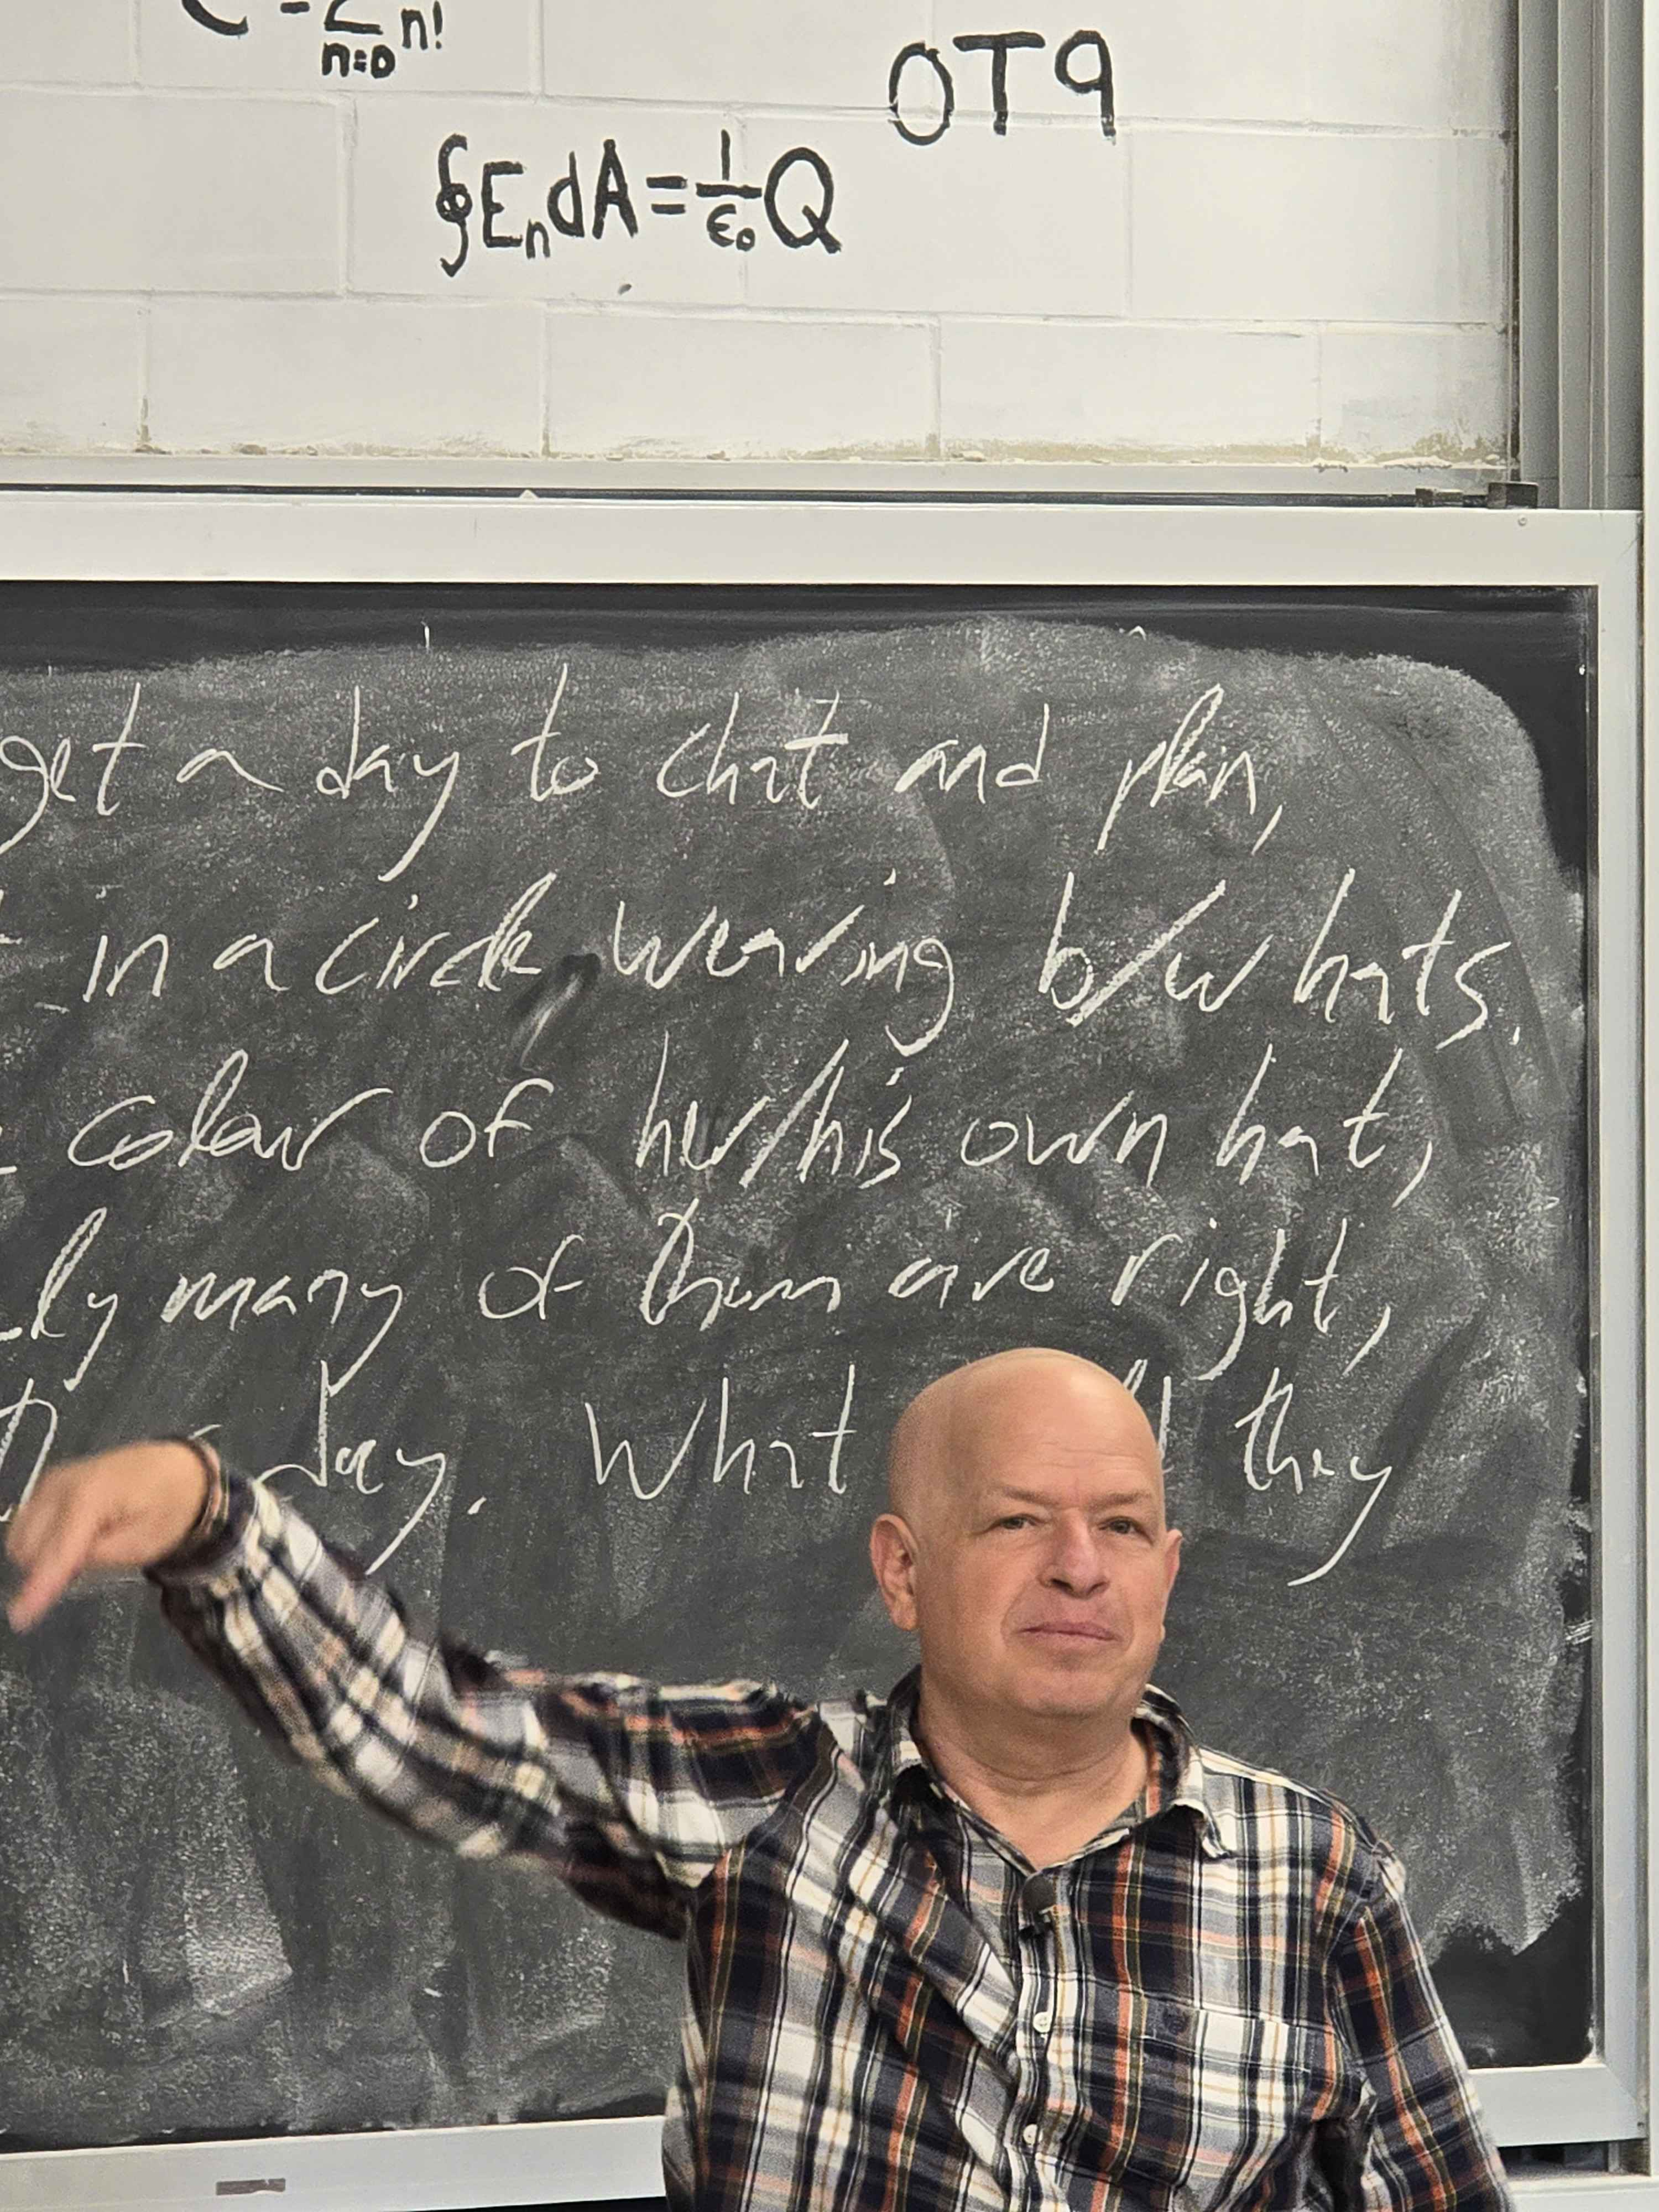
\includegraphics[scale=0.1]{MAT327 Notes/Dror Shirts/dror day 8 shirt.jpg}
\end{figure}

\noindent Recap from last lecture: for any $f : X \to Y$, we have that the following are equivalent:
\begin{enumerate}[label=(\alph*)]
    \item $f$ is continuous.
    \item For all $A \subset X$, we have that $f(\overline{A}) \subset \overline{f(A)}$.
    \item The pre-image of a closed set is closed.
    \item For all $x \in X$ and for all negihborhoods $V$ of $f(x)$, there exists a neighborhood $U$ of $x$ such that $f(U) \subset V$.
\end{enumerate}
Note that we have already established that $(a) \iff (c)$ and $(a) \iff (d)$. We now prove that $(a) \implies (b)$.
\medskip\newline
\noindent Take $x$ in the closure of $A$, and pick a neighborhood $U$ of $f(x)$. Then $f^{-1}(U)$ is open (by continuity), and it contains $x$. Thus, $f^{-1}(U)$ intersects $A$. Let us pick $y \in f^{-1}(U) \cap A$; then we have $f(y) \in U \cap f(A)$, and so every neighborhood of $f(x)$ intersects $f(A)$, and so $f(x) \in \overline{f(A)}$. \qed

\newpage
\noindent As an example, let us $X = \RR^2$, and consider $A = \{(x, \frac{1}{x}) \mid x \neq 0\}$. Then if we let $f$ be the function projecting $A$ to the $x$-axis, i.e. $f(A) = \RR \setminus \{0\}$, and we have that
\[ f(\overline{A}) = f(A) = \RR \setminus\{0\} \subsetneq \overline{f(A)} = \RR. \]
We now continue on our previous claim, and show that $(b) \implies (c)$. Let $B \in Y$ be a closed set, and let $f^{-1}(B) =: A$. Then we may write,
\[ f(\overline{A}) \stackrel{(b)}{\subset} \overline{f(A)} = \overline{f(f^{-1}(B))} \subset \overline{B} = B, \]
since the closure of a closed set is itself. Thus, we have that $\overline{A} \subset f^{-1}(B) = A$, implying $\overline{A} = A$, and so $A$ is closed, i.e. the pre-image of $B$ is closed. \qed
\medskip\newline
\noindent We now move onto infinite products. Suppose $X_\alpha$ is a set for every $\alpha \in I$, and let $X = \prod X_\alpha = \{ x : I \to \bigcup_\alpha X_\alpha \mid \forall \alpha \in I, x(\alpha) \in X_\alpha \}$\footnote{alternatively, the function $x$ can be seen as just a ``collection'' of $x_\alpha$s.}. Per the axiom of choice (which we will refer to as \textit{AC} from now on), if all $X_\alpha$s are not empty, then $X = \prod X_\alpha$ is non-empty.

\medskip
\noindent Assuming AC, we have that $\prod_{\emptyset \neq A \subset \RR} A$ is non-empty. Let us consider the function $c : \SP(\RR) \setminus \{ \emptyset \} \to \RR$ such that $c(A) \in A$. There exists a function on the nonempty sets of reals that picks an element from each set of reals.
\medskip\newline
Let $S = \RR^\NN = \{(a_i)+{i \in \NN} \mid a_i \in \RR\}$. Then we claim that there exists a function $h : S \to S$ such that
\begin{enumerate}[label=(\alph*)]
    \item $h(a)$ depends only on the tail of $a$, meaning if $a \sim b$ (i.e. they have the same tail, meaning $\exists N \in \NN$ such that for all $n > N$, $a_n = b_n$), then $h(a) = h(b)$.
    \item $h(a) \sim a$, i.e. they only differ in finitely many coordinates, and are equal past some index $N$.
\end{enumerate}
\begin{simpleclaim}
    If such a function exists, we can save infinitely many prisoners; recall that the prisoner problem is that every prisoner is given a white or black hat (they cannot see their own hat), and they have to call the color of their own hat out.
\end{simpleclaim}
\noindent Assuming AC, we know that $h$ exists, and so by property (b) of $h$, only finitely many prisoners will die.
\medskip\newline
Let $I = S/\sim$ (read: equivalence classes as per $\sim$ defined earlier, in $S$), and consider $X = \prod_{\alpha \in I} \alpha \ni h'$. Let $h'$ be a function taking the tail of $\alpha$ that finds another sequence whose tail is the same as $\alpha$'s. Then $h(a) = h'(\text{tail of }\alpha)$; unfortunately, to find $h'$, we need to use AC. \qed
\medskip\newline
\noindent Suppose $X_\alpha$ is a topological space, and we want a topology on $X = \prod X_\alpha$. We may approach this in two ways:
\begin{enumerate}
    \item We may choose to generalize the construction,
    \[ \SB = \left\{\prod_{\alpha \in I} U_\alpha \mid \forall \alpha, U_\alpha \subset X_\alpha\right\}, \]
    where each $U_\alpha$ is open. \textit{(We note that this is a dead end.)}
    \item Alternatively, we may generalize the requirements. We want a topology such that:
    \begin{enumerate}[label=(\alph*)]
        \item $\forall \alpha, \prod_\alpha : X \to X_\alpha$, i.e. $\prod_\alpha(x) = x(\alpha) = x_\alpha$
        \item If $g : Z \to X$ has that $\forall \alpha, \pi_\alpha \circ g$ is continuous, then $g$ is continuous.
    \end{enumerate}
\end{enumerate}

\newpage
\begin{simpleclaim}
    There exists a unique topology on $X$ satisfying properties $1$ and $2$.
\end{simpleclaim}
\noindent Observe that at least $\prod_\alpha^{-1} (U_\alpha)$ must be open for every $U_\alpha$, where $\alpha \in I$, to be open in $X$. Let's start by defining
\begin{align*}
    \SB &= \{\pi_{\alpha_1}^{-1} (U_{\alpha_1}) \cap \dots \cap \pi_{\alpha_n}^{-1} (U_{\alpha_n}) \mid \alpha_1, \dots, \alpha_n \in I; \, U_{\alpha_i} \text{ open in } X_i \}; \\
    \SB_\mathrm{cyl} &= \left\{ \prod_{\alpha \in I} U_\alpha \mid \forall \alpha, U_\alpha \subset X_\alpha \text{ is open}; \, U_\alpha = X_\alpha \text{ for all but finitely many } \alpha \text{'s.} \right\}.
\end{align*}
This is exactly the previous basis $\SB$ (note that we read cyl as cylinder here\footnote{and i have no idea why it's cylinder, but we play along for now}). We claim that this works; observe that
\begin{enumerate}[label=(\alph*)]
    \item $\SB_\mathrm{cyl}$ is indeed a basis, so let $\ST_\mathrm{cyl}$ be the topology it generates, meaning that property $1$ holds,
    \item We also have that property $2$ holds; assume $g : Z \to X$ and $\pi_\alpha \circ g$ is continuous for all $\alpha$. Then let us write,
    \[ g^{-1} \left( \bigcap_{i=1}^n \pi_{\alpha_i}^{-1} (U_{\alpha_i}) \right) = \bigcap_{i=1}^n g^{-1} (\pi_\alpha^{-1} (U_{\alpha_i})) = \bigcap_{i=1}^n (\pi_\alpha \circ g)^{-1} (U_{\alpha_i}). \]
    Since each $\pi_\alpha \circ g$ is assumed to be continuous, we have that this is a finite intersection of open sets, and we conclude that the above is indeed open.
\end{enumerate}
Now that we have proved existence, we claim that we also have uniqueness. If $\ST'$ and $\ST''$ are topologies on $X = \prod X_\alpha$ satisfying $1$ and $2$, then $\ST' = \ST''$; to start, consider the identity map $g = \mathrm{id}$,
\[ \left(\prod X_\alpha, \ST' \right) \xrightarrow[]{\mathrm{id}} \left(\prod X_\alpha, \ST'' \right). \]
Then $\pi_\alpha \circ g = \pi_\alpha \circ \mathrm{id} = \pi_\alpha$ is continuous by property $1$ of $\ST'$; thus, by property $2$ of $\ST''$, we see that the identity map is continuous, and we proceed as per our previous uniqueness proofs to see that $\ST' = \ST''$. \qed
\medskip\newline
For concreteness, we now present an example. Let $c : \RR \to \RR^\NN$, where $c(t) = (t, t, \dots)$, i.e. the constant sequence consisting of $t$s. Then $c : \RR \to \RR^\NN_\mathrm{cyl}$ is continuous. $(\pi_k \circ c)(t) = t$ (since $c = \mathrm{id}_\RR$), and so $c$ is continuous.
\medskip\newline
Now, consider $c : \RR \to \RR^\NN_\mathrm{box}$. Then
\[c^{-1} \left(\prod_{k \in \NN} \left(-\frac{1}{k}, \frac{1}{k}\right)\right) = \{0\}, \]
which is not open.
\medskip\newline
Note that $\ST_\mathrm{box} \neq \ST_\mathrm{cyl}$. In fact, the cylinder topology is contained in the box topology, and the inclusion is not an equality, $\ST_\mathrm{cyl} \subsetneq \ST_\mathrm{box}$. In both topologies,
\begin{enumerate}[label=(\alph*)]
    \item If $A_\alpha \subset X_\alpha$, for every $\alpha$, $\prod A_\alpha$ as a subset of a product is the same as $\prod A_\alpha$ as a product of subsets. \textit{(The proof is messy. We leave it alone for now.)}
    \item If, for all $\alpha$, $X_\alpha$ is $T_2$, then $(\prod_\alpha X_\alpha)_\mathrm{box}, (\prod_\alpha X_\alpha)_\mathrm{cyl}$ are $T_2$.
\end{enumerate}